\documentclass{standalone}
\usepackage{tikz}
\usetikzlibrary{patterns, positioning}
\usepackage[sfdefault]{ClearSans} %% option 'sfdefault' activates Clear Sans as the default text font
\usepackage[T1]{fontenc}

\begin{document}
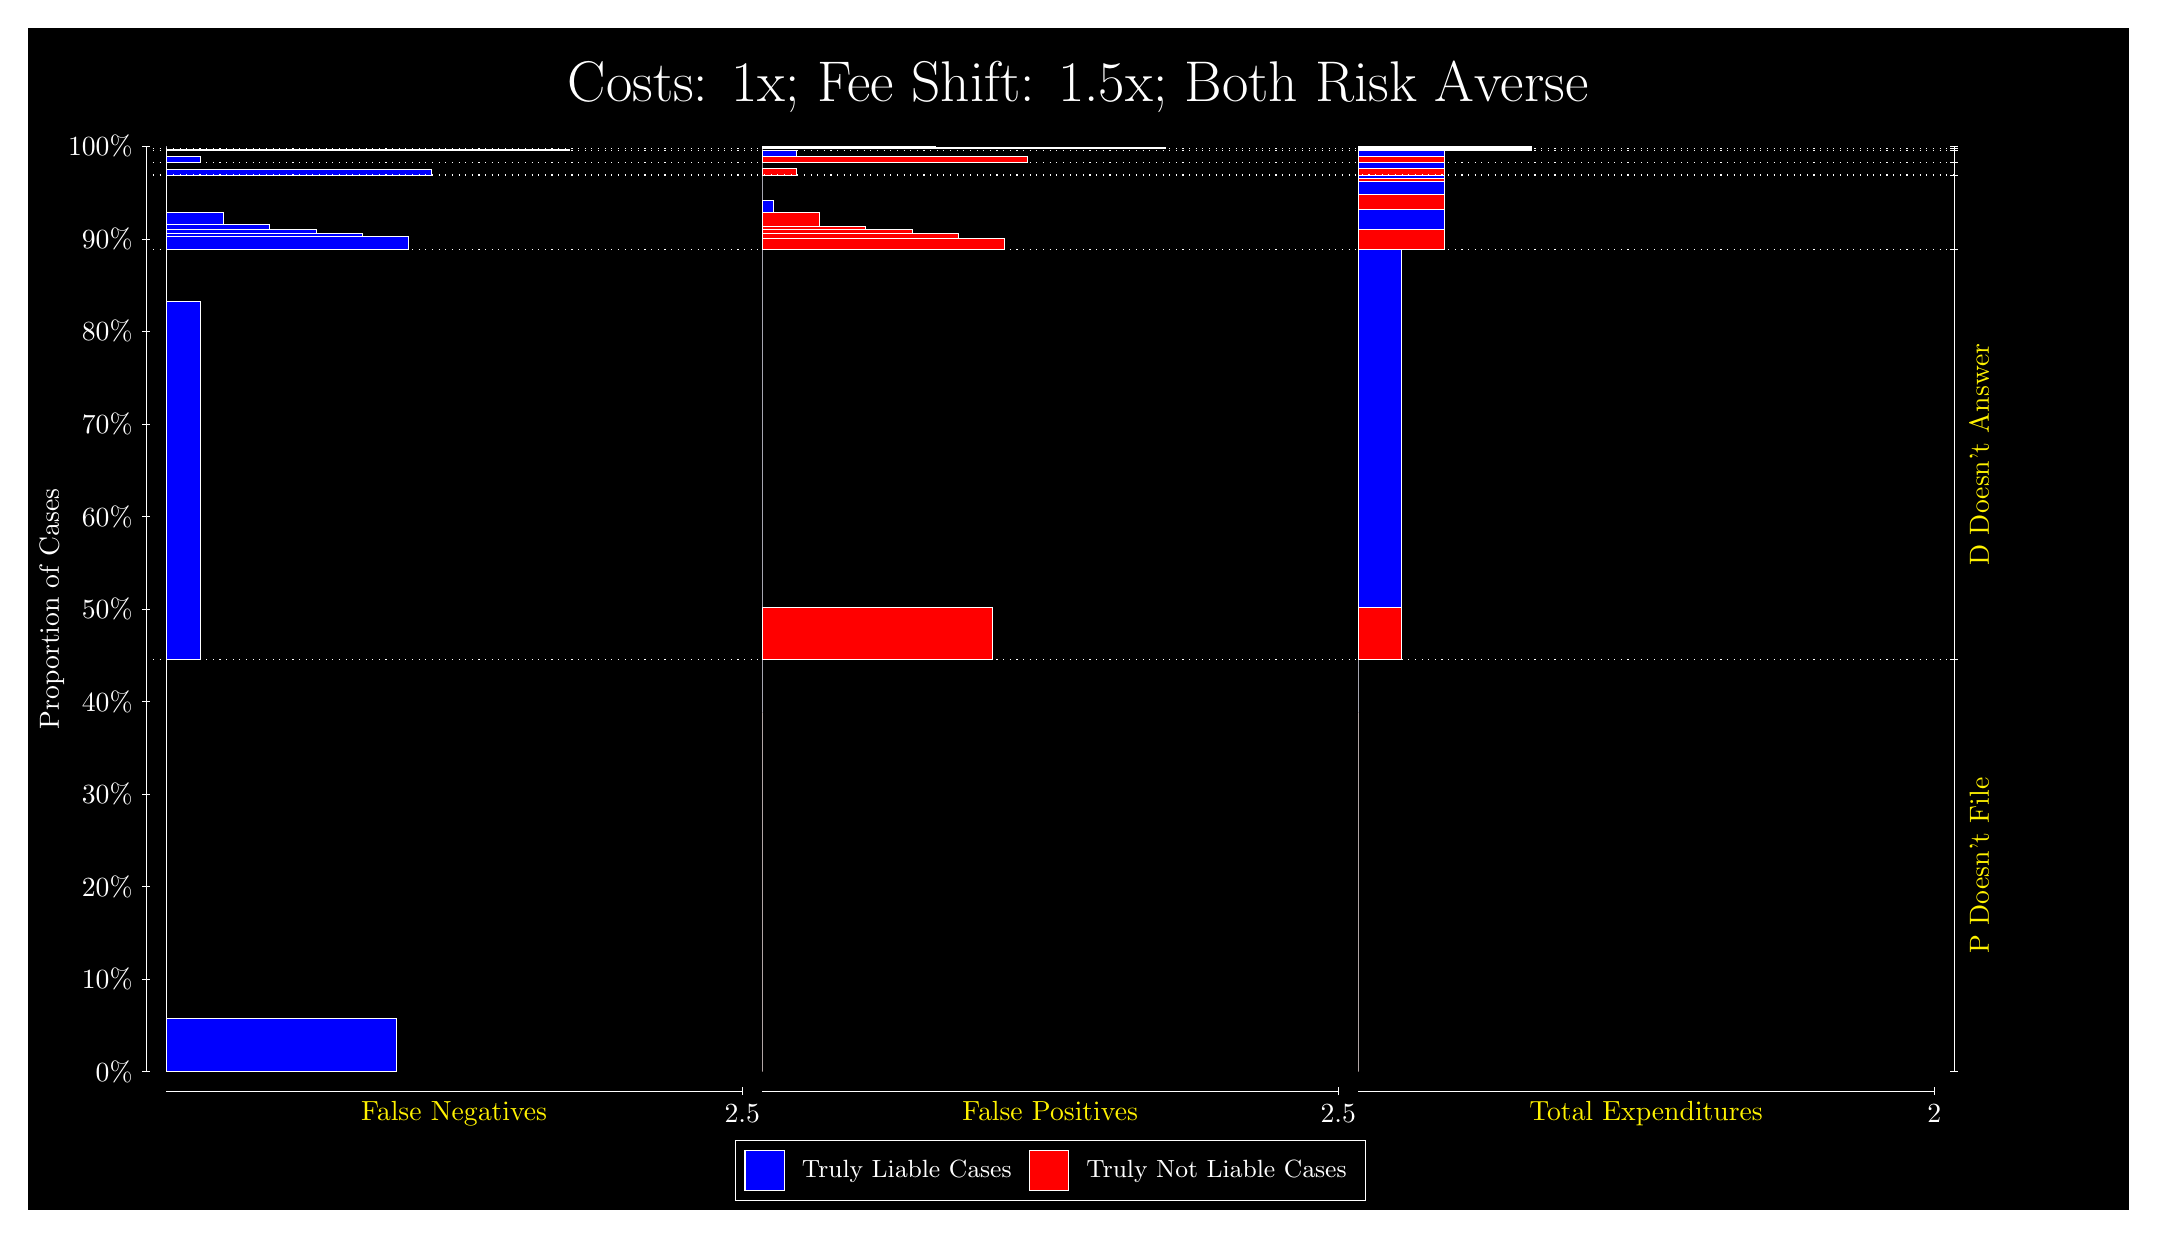
\begin{tikzpicture}
\draw[fill=black] (0,0) rectangle (26.667,15);
\draw[text=white] (0,13.5) rectangle (26.667,15) node[midway] {\huge Costs: 1x; Fee Shift: 1.5x; Both Risk Averse};
\draw[white, very thin] (1.5,1.75) -- (1.5,13.5);
\node[rotate=90, text=white, anchor=center] at (0.3, 7.625) {Proportion of Cases};
\draw[white, very thin] (1.45,1.75) -- (1.55,1.75);
\node[text=white, anchor=east] at (1.45, 1.75) {0\%};
\draw[white, very thin] (1.45,2.925) -- (1.55,2.925);
\node[text=white, anchor=east] at (1.45, 2.925) {10\%};
\draw[white, very thin] (1.45,4.1) -- (1.55,4.1);
\node[text=white, anchor=east] at (1.45, 4.1) {20\%};
\draw[white, very thin] (1.45,5.275) -- (1.55,5.275);
\node[text=white, anchor=east] at (1.45, 5.275) {30\%};
\draw[white, very thin] (1.45,6.45) -- (1.55,6.45);
\node[text=white, anchor=east] at (1.45, 6.45) {40\%};
\draw[white, very thin] (1.45,7.625) -- (1.55,7.625);
\node[text=white, anchor=east] at (1.45, 7.625) {50\%};
\draw[white, very thin] (1.45,8.8) -- (1.55,8.8);
\node[text=white, anchor=east] at (1.45, 8.8) {60\%};
\draw[white, very thin] (1.45,9.975) -- (1.55,9.975);
\node[text=white, anchor=east] at (1.45, 9.975) {70\%};
\draw[white, very thin] (1.45,11.15) -- (1.55,11.15);
\node[text=white, anchor=east] at (1.45, 11.15) {80\%};
\draw[white, very thin] (1.45,12.325) -- (1.55,12.325);
\node[text=white, anchor=east] at (1.45, 12.325) {90\%};
\draw[white, very thin] (1.45,13.5) -- (1.55,13.5);
\node[text=white, anchor=east] at (1.45, 13.5) {100\%};

\draw[white, very thin] (24.457,1.75) -- (24.457,13.5);
\draw[white, very thin] (24.407,1.75) -- (24.507,1.75);
\node[anchor=west] at (24.407, 1.75) {};
\draw[white, very thin] (24.407,6.9852) -- (24.507,6.9852);
\node[anchor=west] at (24.407, 6.9852) {};
\draw[white, very thin] (24.407,12.187) -- (24.507,12.187);
\node[anchor=west] at (24.407, 12.187) {};
\draw[white, very thin] (24.407,13.136) -- (24.507,13.136);
\node[anchor=west] at (24.407, 13.136) {};
\draw[white, very thin] (24.407,13.296) -- (24.507,13.296);
\node[anchor=west] at (24.407, 13.296) {};
\draw[white, very thin] (24.407,13.451) -- (24.507,13.451);
\node[anchor=west] at (24.407, 13.451) {};
\draw[white, very thin] (24.407,13.475) -- (24.507,13.475);
\node[anchor=west] at (24.407, 13.475) {};
\draw[white, very thin] (24.407,13.5) -- (24.507,13.5);
\node[anchor=west] at (24.407, 13.5) {};

\draw[white, very thin, fill=blue] (1.75,1.75) rectangle (4.6775,2.4235);
\draw[white, very thin, fill=red] (1.75,2.4235) rectangle (1.75,6.9852);
\draw[white, very thin, fill=blue] (1.75,6.9852) rectangle (2.1891,11.53);
\draw[white, very thin, fill=red] (1.75,11.53) rectangle (1.75,12.187);
\draw[white, very thin, fill=blue] (1.75,12.187) rectangle (4.8239,12.361);
\draw[white, very thin, fill=blue] (1.75,12.361) rectangle (4.2384,12.4);
\draw[white, very thin, fill=blue] (1.75,12.4) rectangle (3.6529,12.441);
\draw[white, very thin, fill=blue] (1.75,12.441) rectangle (3.0674,12.504);
\draw[white, very thin, fill=blue] (1.75,12.504) rectangle (2.4819,12.662);
\draw[white, very thin, fill=red] (1.75,12.662) rectangle (1.75,13.136);
\draw[white, very thin, fill=blue] (1.75,13.136) rectangle (5.1167,13.21);
\draw[white, very thin, fill=red] (1.75,13.21) rectangle (1.75,13.296);
\draw[white, very thin, fill=blue] (1.75,13.296) rectangle (2.1891,13.379);
\draw[white, very thin, fill=red] (1.75,13.379) rectangle (1.75,13.451);
\draw[white, very thin, fill=blue] (1.75,13.451) rectangle (6.8732,13.459);
\draw[white, very thin, fill=red] (1.75,13.459) rectangle (1.75,13.475);
\draw[white, very thin, fill=red] (1.75,13.475) rectangle (1.75,13.483);
\draw[white, very thin, fill=blue] (1.75,13.483) rectangle (1.75,13.5);
\draw[white, very thin, fill=red] (9.3189,1.75) rectangle (9.3189,6.3118);
\draw[white, very thin, fill=blue] (9.3189,6.3118) rectangle (9.3189,6.9852);
\draw[white, very thin, fill=red] (9.3189,6.9852) rectangle (12.246,7.642);
\draw[white, very thin, fill=blue] (9.3189,7.642) rectangle (9.3189,12.187);
\draw[white, very thin, fill=red] (9.3189,12.187) rectangle (12.393,12.337);
\draw[white, very thin, fill=red] (9.3189,12.337) rectangle (11.807,12.4);
\draw[white, very thin, fill=red] (9.3189,12.4) rectangle (11.222,12.441);
\draw[white, very thin, fill=red] (9.3189,12.441) rectangle (10.636,12.48);
\draw[white, very thin, fill=red] (9.3189,12.48) rectangle (10.051,12.662);
\draw[white, very thin, fill=blue] (9.3189,12.662) rectangle (9.4652,12.82);
\draw[white, very thin, fill=blue] (9.3189,12.82) rectangle (9.3189,13.136);
\draw[white, very thin, fill=red] (9.3189,13.136) rectangle (9.758,13.222);
\draw[white, very thin, fill=blue] (9.3189,13.222) rectangle (9.3189,13.296);
\draw[white, very thin, fill=red] (9.3189,13.296) rectangle (12.686,13.368);
\draw[white, very thin, fill=blue] (9.3189,13.368) rectangle (9.758,13.451);
\draw[white, very thin, fill=red] (9.3189,13.451) rectangle (9.3189,13.467);
\draw[white, very thin, fill=blue] (9.3189,13.467) rectangle (9.3189,13.475);
\draw[white, very thin, fill=red] (9.3189,13.475) rectangle (14.442,13.483);
\draw[white, very thin, fill=blue] (9.3189,13.483) rectangle (11.515,13.5);
\draw[white, very thin, fill=red] (16.888,1.75) rectangle (16.888,6.3118);
\draw[white, very thin, fill=blue] (16.888,6.3118) rectangle (16.888,6.9852);
\draw[white, very thin, fill=red] (16.888,6.9852) rectangle (17.437,7.642);
\draw[white, very thin, fill=blue] (16.888,7.642) rectangle (17.437,12.187);
\draw[white, very thin, fill=red] (16.888,12.187) rectangle (17.986,12.441);
\draw[white, very thin, fill=blue] (16.888,12.441) rectangle (17.986,12.703);
\draw[white, very thin, fill=red] (16.888,12.703) rectangle (17.986,12.885);
\draw[white, very thin, fill=blue] (16.888,12.885) rectangle (17.986,13.059);
\draw[white, very thin, fill=red] (16.888,13.059) rectangle (17.986,13.098);
\draw[white, very thin, fill=blue] (16.888,13.098) rectangle (17.986,13.136);
\draw[white, very thin, fill=red] (16.888,13.136) rectangle (17.986,13.222);
\draw[white, very thin, fill=blue] (16.888,13.222) rectangle (17.986,13.296);
\draw[white, very thin, fill=red] (16.888,13.296) rectangle (17.986,13.368);
\draw[white, very thin, fill=blue] (16.888,13.368) rectangle (17.986,13.451);
\draw[white, very thin, fill=red] (16.888,13.451) rectangle (19.083,13.467);
\draw[white, very thin, fill=blue] (16.888,13.467) rectangle (19.083,13.475);
\draw[white, very thin, fill=red] (16.888,13.475) rectangle (19.083,13.483);
\draw[white, very thin, fill=blue] (16.888,13.483) rectangle (19.083,13.5);
\draw[white, dotted] (1.5,6.9852) -- (24.457,6.9852);
\draw[white, dotted] (1.5,12.187) -- (24.457,12.187);
\draw[white, dotted] (1.5,13.136) -- (24.457,13.136);
\draw[white, dotted] (1.5,13.296) -- (24.457,13.296);
\draw[white, dotted] (1.5,13.451) -- (24.457,13.451);
\draw[white, dotted] (1.5,13.475) -- (24.457,13.475);
\draw[white, very thin] (1.75,1.5) -- (9.0689,1.5);
\node[text=yellow, anchor=north] at (5.4094, 1.5) {False Negatives};
\draw[white, very thin] (9.0689,1.45) -- (9.0689,1.55);
\node[text=white, anchor=north] at (9.0689, 1.45) {2.5};

\draw[white, very thin] (9.3189,1.5) -- (16.638,1.5);
\node[text=yellow, anchor=north] at (12.978, 1.5) {False Positives};
\draw[white, very thin] (16.638,1.45) -- (16.638,1.55);
\node[text=white, anchor=north] at (16.638, 1.45) {2.5};

\draw[white, very thin] (16.888,1.5) -- (24.207,1.5);
\node[text=yellow, anchor=north] at (20.547, 1.5) {Total Expenditures};
\draw[white, very thin] (24.207,1.45) -- (24.207,1.55);
\node[text=white, anchor=north] at (24.207, 1.45) {2};

\node[text=yellow, centered, rotate=90] at (24.777, 4.3676) {P Doesn't File};
\node[text=yellow, centered, rotate=90] at (24.777, 9.5861) {D Doesn't Answer};






\draw (12.978300999999998,1.5) node[draw=none] (baseCoordinate) {};
\begin{scope}[align=center]
        \matrix[scale=0.5, draw=white, below=0.5cm of baseCoordinate, nodes={draw}, column sep=0.1cm]{
            \node[rectangle, draw, minimum width=0.5cm, minimum height=0.5cm, fill=blue] {}; &
            \node[draw=none, font=\small, text=white] (B) {Truly Liable Cases}; &
            \node[rectangle, draw, minimum width=0.5cm, minimum height=0.5cm, fill=red] {}; &
            \node[draw=none, font=\small, text=white] (B) {Truly Not Liable Cases}; \\
            };
\end{scope}

\end{tikzpicture}
\end{document}